\begin{frame}
	\myheading{Module 13.4 : Finding influence of input pixels using backpropagation}
\end{frame}

%%%%%%%%%%%%%%%%%%%%%%%%%%%%%%%%%%%%%%%%%%%%%%%%%%%%%%%%%%%%%%%%%%%%%%%%%%%%%%%%%%%%%%%%%

\begin{frame}
	\begin{columns}
		\column{0.5\textwidth}
		\centering
		% \begin{figure}
		% 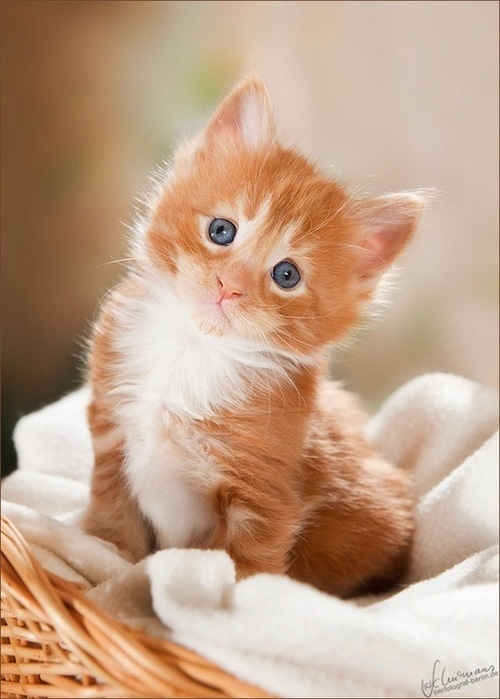
\includegraphics[scale=0.17,trim={0 2cm 0 3cm},clip=true]{images/CatImage.jpg}
		% \end{figure}
			
		\begin{tikzpicture}[scale=0.8,transform shape]

\tikzstyle{input_neuron}=[circle,draw=red!50,fill=red!10,thick,minimum size=5mm]
\tikzstyle{input_neuron1}=[circle,draw=yellow!50,fill=yellow,thick,minimum size=5mm]
\tikzstyle{hidden_neuron}=[circle,draw=blue!50,fill=cyan!10,thick,minimum size=5mm]
\tikzstyle{hidden_neuron1}=[circle,draw=yellow!50,fill=yellow,thick,minimum size=5mm]
\tikzstyle{output_neuron}=[circle,draw=green!50,fill=green!10,thick,minimum size=5mm]
\tikzstyle{bias_neuron}=[circle,draw=red!50,fill=red!10,thick,minimum size=2mm]
\tikzstyle{bias_hidden_neuron}=[circle,draw=blue!50,fill=cyan!10,thick,minimum size=2mm]
\tikzstyle{bias_hidden_neuron_hi}=[circle,draw=orange,fill=cyan!10,thick,minimum size=2mm]
\tikzstyle{bias_hidden_neuron_hi_old}=[circle,draw=yellow,fill=cyan!10,thick,minimum size=2mm]
\tikzstyle{input}=[circle,draw=black!50,fill=black!20,thick,minimum size=6mm]

\node [input_neuron] (B) at (-4.0,1){};
\node [input_neuron] (C) at (-3,1){};
\node [input_neuron] (D) at (-2,1){};
\node [input_neuron] (E) at (-1,1){};
\node [input_neuron] (F) at (0,1){};
\node [input_neuron] (G) at (1,1){};
\only<1->{\node [input_neuron] (H) at (2,1){};}
\only<2->{\node [input_neuron1] (H) at (2,1){\tiny $x_i$};}
\node [input_neuron] (I) at (3,1){};
\node [input_neuron] (J) at (4,1){};


\node [rectangle, draw=red, minimum width=90mm, minimum height=6mm] at (0,1){};
\node [hidden_neuron] (O) at (2,2.7){};
\node [hidden_neuron] (N) at (1,2.7){};
\node [hidden_neuron] (M) at (-1,2.7){};
\node [hidden_neuron] (L) at (-2,2.7){};


\node [hidden_neuron] (Oo) at (-3,4){};
\node [hidden_neuron] (Nn) at (-2,4){};
\node [hidden_neuron] (Mm) at (-1,4){};
\only<2->{\node [hidden_neuron1] (Zz) at (0,4){\tiny $h_j$};}
\only<1>{\node [hidden_neuron] (Zz) at (0,4){};}
\node [hidden_neuron] (Ll) at (1,4){};
\node [hidden_neuron] (Xx) at (2,4){};
\node [hidden_neuron] (Yy) at (3,4){};

\node [output_neuron] (To) at (2,5.3){};
\node [output_neuron] (Tp) at (1,5.3){};
\node [output_neuron] (Tq) at (0,5.3){};
\node [output_neuron] (Tr) at (-1,5.3){};
\node [output_neuron] (Ts) at (-2,5.3){};
\onslide<1->{
	
	\draw [->] (B) -- (L);
	\draw [->] (C) -- (L);

	\draw [->] (E) -- (L);




	\draw [->] (C) -- (M);
	\draw [->] (D) -- (M);

	\draw [->] (F) -- (M);
	\draw [->] (G) -- (M);
	\draw [->] (E) -- (N);
	\draw [->] (F) -- (N);
	\draw [->] (H) -- (N);
	\draw [->] (I) -- (N);


	\draw [->] (F) -- (O);
	\draw [->] (G) -- (O);
	\draw [->] (I) -- (O);
	\draw [->] (J) -- (O);

	\draw [->] (L) -- (Oo);
	
	\draw [->] (L) -- (Nn);	
	
	\draw [->] (L) -- (Xx);
	\draw [->] (L) -- (Yy);
	\draw [->] (L) -- (Zz);



	\draw [->] (M) -- (Oo);
	\draw [->] (M) -- (Mm);	
	
	\draw [->] (M) -- (Ll);
	\draw [->] (M) -- (Xx);
	\draw [->] (M) -- (Yy);
	



	
	\draw [->] (N) -- (Mm);	
	\draw [->] (N) -- (Nn);	
	
	\draw [->] (N) -- (Xx);
	
	\draw [->] (N) -- (Zz);



	
	\draw [->] (O) -- (Mm);	
	\draw [->] (O) -- (Nn);	
	
	\draw [->] (O) -- (Xx);
	\draw [->] (O) -- (Yy);
	
	\draw [->] (Ll) -- (To);
	\draw [->] (Ll) -- (Tp);
	\draw [->] (Ll) -- (Tq);
	\draw [->] (Ll) -- (Tr);
	\draw [->] (Ll) -- (Ts);


	\draw [->] (Mm) -- (To);
	\draw [->] (Mm) -- (Tp);
	\draw [->] (Mm) -- (Tq);
	\draw [->] (Mm) -- (Tr);
	\draw [->] (Mm) -- (Ts);

	\draw [->] (Nn) -- (To);
	\draw [->] (Nn) -- (Tp);
	\draw [->] (Nn) -- (Tq);
	\draw [->] (Nn) -- (Tr);
	\draw [->] (Nn) -- (Ts);

	\draw [->] (Mm) -- (To);
	\draw [->] (Mm) -- (Tp);
	\draw [->] (Mm) -- (Tq);
	\draw [->] (Mm) -- (Tr);
	\draw [->] (Mm) -- (Ts);

	\draw [->] (Nn) -- (To);
	\draw [->] (Nn) -- (Tp);
	\draw [->] (Nn) -- (Tq);
	\draw [->] (Nn) -- (Tr);
	\draw [->] (Nn) -- (Ts);


	\draw [->] (Oo) -- (To);
	\draw [->] (Oo) -- (Tp);
	\draw [->] (Oo) -- (Tq);
	\draw [->] (Oo) -- (Tr);
	\draw [->] (Oo) -- (Ts);

	\draw [->] (Xx) -- (To);
	\draw [->] (Xx) -- (Tp);
	\draw [->] (Xx) -- (Tq);
	\draw [->] (Xx) -- (Tr);
	\draw [->] (Xx) -- (Ts);

	\draw [->] (Yy) -- (To);
	\draw [->] (Yy) -- (Tp);
	\draw [->] (Yy) -- (Tq);
	\draw [->] (Yy) -- (Tr);
	\draw [->] (Yy) -- (Ts);



	\draw [->] (Zz) -- (To);
	\draw [->] (Zz) -- (Tp);
	\draw [->] (Zz) -- (Tq);
	\draw [->] (Zz) -- (Tr);
	\draw [->] (Zz) -- (Ts);

	\draw [->, line width=2, color=red] (0,-0.2)-- (0,0.75);
	\node [] at (1,0.25){\footnotesize flatten};
}
\onslide<1->{
	
	\draw [->,color=blue] (B) -- (L);
	\draw [->,color=blue] (C) -- (L);

	\draw [->,color=blue] (E) -- (L);
	\draw [->,color=blue] (F) -- (L);

}

\onslide<1->{
	
	\draw [->,color=blue] (C) -- (M);
	\draw [->,color=blue] (D) -- (M);

	\draw [->,color=blue] (F) -- (M);
	\draw [->,color=blue] (G) -- (M);
}

\onslide<1->{
	
	\draw [->,color=blue] (E) -- (N);
	\draw [->,color=blue] (F) -- (N);

	\draw [->,color=blue] (H) -- (N);
	\draw [->,color=blue] (I) -- (N);


}

\onslide<1->{
	
	\draw [->,color=blue] (F) -- (O);
	\draw [->,color=blue] (I) -- (O);

	\draw [->,color=blue] (G) -- (O);
	\draw [->,color=blue] (J) -- (O);


}
\end{tikzpicture}


		%\vspace{-0.5cm}
		\begin{tikzpicture}
	\node at (+0.0,-0.0) (cat)  { 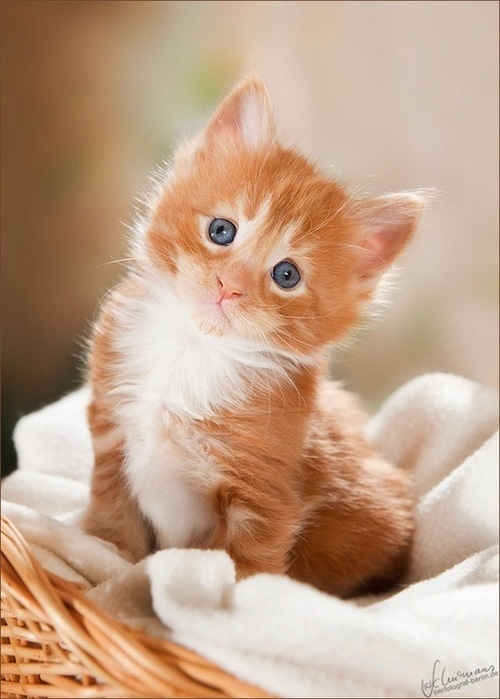
\includegraphics[scale=0.17,trim={0 3.9cm 0 3cm},clip=true,height=3cm]{images/CatImage.jpg}};
	\draw[step=0.5cm,color=gray] (-1.5,-1.5) grid (1.5,1.5);
	\foreach \y in {+0.75,+0.25,-0.25,-0.75}
	\foreach \x in {-0.75,-0.25,0.25,0.75}
	\node at (\x,\y) {$\cdot$};
			
	\foreach \x in {-0.25,0.25,0.75,1.25}
	\node at (\x,1.25) {$\cdot$};
	
	\foreach \x in {-1.25,-0.75,-0.25,0.25,0.75}
	\node at (\x,-1.25) {$\cdot$};
	
	\foreach \y in {-0.75,-0.25,0.25,0.75}{
		\node at (1.25,\y) {$\cdot$};
		\node at (-1.25,\y) {$\cdot$};
	}
	\node at (-1.25,+1.25) {\footnotesize{$x_0$}};
	\node at (-0.75,+1.25) {\footnotesize{$x_1$}};
	\node at (+1.25,-1.25) {\footnotesize{$x_{mn}$}};
			
\end{tikzpicture}	
			
		\column{0.5\textwidth}
		\begin{overlayarea}{\textwidth}{\textheight}
			\begin{itemize}
				\justifying
				\onslide<1->{\item We can think of an image as a $m \times n$ inputs $x_0,x_1,\ldots, x_{m \times n}$}
				\onslide<2->{\item We are interested in finding the influence of each of these inputs($x_i$) on a given neuron($h_j$) }
				\onslide<3->{\item If a small change in $x_i$ causes a large change in $h_j$ then we can say that $x_i$ has a lot of influence of $h_j$}
				\onslide<4->{\item In other words the gradient $\frac{\partial h_j}{\partial x_i}$ could tell us about the influence}
			\end{itemize}
		\end{overlayarea}
	\end{columns}
\end{frame}

%%%%%%%%%%%%%%%%%%%%%%%%%%%%%%%%%%%%%%%%%%%%%%%%%%%%%%%%%%%%%%%%%%%%%%%%%%%%%%%%%%%%%%%%%

\begin{frame}
	\begin{columns}
		\column{0.5\textwidth}
		\centering
		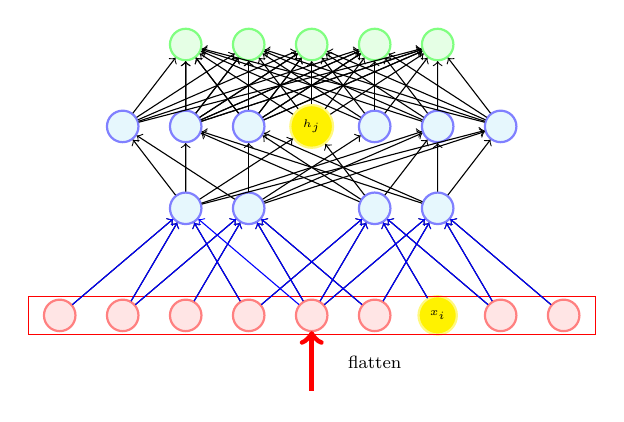
\begin{tikzpicture}[scale=0.8,transform shape]

	\tikzstyle{input_neuron}=[circle,draw=red!50,fill=red!10,thick,minimum size=5mm]
	\tikzstyle{input_neuron1}=[circle,draw=yellow!50,fill=yellow,thick,minimum size=5mm]
	\tikzstyle{hidden_neuron}=[circle,draw=blue!50,fill=cyan!10,thick,minimum size=5mm]
	\tikzstyle{hidden_neuron1}=[circle,draw=yellow!50,fill=yellow,thick,minimum size=5mm]
	\tikzstyle{output_neuron}=[circle,draw=green!50,fill=green!10,thick,minimum size=5mm]
	\tikzstyle{bias_neuron}=[circle,draw=red!50,fill=red!10,thick,minimum size=2mm]
	\tikzstyle{bias_hidden_neuron}=[circle,draw=blue!50,fill=cyan!10,thick,minimum size=2mm]
	\tikzstyle{bias_hidden_neuron_hi}=[circle,draw=orange,fill=cyan!10,thick,minimum size=2mm]
	\tikzstyle{bias_hidden_neuron_hi_old}=[circle,draw=yellow,fill=cyan!10,thick,minimum size=2mm]
	\tikzstyle{input}=[circle,draw=black!50,fill=black!20,thick,minimum size=6mm]
	
	\node [input_neuron] (B) at (-4.0,1){};
	\node [input_neuron] (C) at (-3,1){};
	\node [input_neuron] (D) at (-2,1){};
	\node [input_neuron] (E) at (-1,1){};
	\node [input_neuron] (F) at (0,1){};
	\node [input_neuron] (G) at (1,1){};
	\node [input_neuron1] (H) at (2,1){\tiny $x_i$};
	\node [input_neuron] (I) at (3,1){};
	\node [input_neuron] (J) at (4,1){};
	
	
	\node [rectangle, draw=red, minimum width=90mm, minimum height=6mm] at (0,1){};
	\node [hidden_neuron] (O) at (2,2.7){};
	\node [hidden_neuron] (N) at (1,2.7){};
	\node [hidden_neuron] (M) at (-1,2.7){};
	\node [hidden_neuron] (L) at (-2,2.7){};
	
	
	\node [hidden_neuron] (Oo) at (-3,4){};
	\node [hidden_neuron] (Nn) at (-2,4){};
	\node [hidden_neuron] (Mm) at (-1,4){};
	\node [hidden_neuron1] (Zz) at (0,4){\tiny $h_j$};
	
	\node [hidden_neuron] (Ll) at (1,4){};
	\node [hidden_neuron] (Xx) at (2,4){};
	\node [hidden_neuron] (Yy) at (3,4){};
	
	\node [output_neuron] (To) at (2,5.3){};
	\node [output_neuron] (Tp) at (1,5.3){};
	\node [output_neuron] (Tq) at (0,5.3){};
	\node [output_neuron] (Tr) at (-1,5.3){};
	\node [output_neuron] (Ts) at (-2,5.3){};
	\onslide<1->{
		
		\draw [->] (B) -- (L);
		\draw [->] (C) -- (L);
	
		\draw [->] (E) -- (L);
	
	
	
	
		\draw [->] (C) -- (M);
		\draw [->] (D) -- (M);
	
		\draw [->] (F) -- (M);
		\draw [->] (G) -- (M);
		\draw [->] (E) -- (N);
		\draw [->] (F) -- (N);
		\draw [->] (H) -- (N);
		\draw [->] (I) -- (N);
	
	
		\draw [->] (F) -- (O);
		\draw [->] (G) -- (O);
		\draw [->] (I) -- (O);
		\draw [->] (J) -- (O);
	
		\draw [->] (L) -- (Oo);
		
		\draw [->] (L) -- (Nn);	
		
		\draw [->] (L) -- (Xx);
		\draw [->] (L) -- (Yy);
		\draw [->] (L) -- (Zz);
	
	
	
		\draw [->] (M) -- (Oo);
		\draw [->] (M) -- (Mm);	
		
		\draw [->] (M) -- (Ll);
		\draw [->] (M) -- (Xx);
		\draw [->] (M) -- (Yy);
		
	
	
	
		
		\draw [->] (N) -- (Mm);	
		\draw [->] (N) -- (Nn);	
		
		\draw [->] (N) -- (Xx);
		
		\draw [->] (N) -- (Zz);
	
	
	
		
		\draw [->] (O) -- (Mm);	
		\draw [->] (O) -- (Nn);	
		
		\draw [->] (O) -- (Xx);
		\draw [->] (O) -- (Yy);
		
		\draw [->] (Ll) -- (To);
		\draw [->] (Ll) -- (Tp);
		\draw [->] (Ll) -- (Tq);
		\draw [->] (Ll) -- (Tr);
		\draw [->] (Ll) -- (Ts);
	
	
		\draw [->] (Mm) -- (To);
		\draw [->] (Mm) -- (Tp);
		\draw [->] (Mm) -- (Tq);
		\draw [->] (Mm) -- (Tr);
		\draw [->] (Mm) -- (Ts);
	
		\draw [->] (Nn) -- (To);
		\draw [->] (Nn) -- (Tp);
		\draw [->] (Nn) -- (Tq);
		\draw [->] (Nn) -- (Tr);
		\draw [->] (Nn) -- (Ts);
	
		\draw [->] (Mm) -- (To);
		\draw [->] (Mm) -- (Tp);
		\draw [->] (Mm) -- (Tq);
		\draw [->] (Mm) -- (Tr);
		\draw [->] (Mm) -- (Ts);
	
		\draw [->] (Nn) -- (To);
		\draw [->] (Nn) -- (Tp);
		\draw [->] (Nn) -- (Tq);
		\draw [->] (Nn) -- (Tr);
		\draw [->] (Nn) -- (Ts);
	
	
		\draw [->] (Oo) -- (To);
		\draw [->] (Oo) -- (Tp);
		\draw [->] (Oo) -- (Tq);
		\draw [->] (Oo) -- (Tr);
		\draw [->] (Oo) -- (Ts);
	
		\draw [->] (Xx) -- (To);
		\draw [->] (Xx) -- (Tp);
		\draw [->] (Xx) -- (Tq);
		\draw [->] (Xx) -- (Tr);
		\draw [->] (Xx) -- (Ts);
	
		\draw [->] (Yy) -- (To);
		\draw [->] (Yy) -- (Tp);
		\draw [->] (Yy) -- (Tq);
		\draw [->] (Yy) -- (Tr);
		\draw [->] (Yy) -- (Ts);
	
	
	
		\draw [->] (Zz) -- (To);
		\draw [->] (Zz) -- (Tp);
		\draw [->] (Zz) -- (Tq);
		\draw [->] (Zz) -- (Tr);
		\draw [->] (Zz) -- (Ts);
	
		\draw [->, line width=2, color=red] (0,-0.2)-- (0,0.75);
		\node [] at (1,0.25){\footnotesize flatten};
	}
	\onslide<1->{
		
		\draw [->,color=blue] (B) -- (L);
		\draw [->,color=blue] (C) -- (L);
	
		\draw [->,color=blue] (E) -- (L);
		\draw [->,color=blue] (F) -- (L);
	
	}
	
	\onslide<1->{
		
		\draw [->,color=blue] (C) -- (M);
		\draw [->,color=blue] (D) -- (M);
	
		\draw [->,color=blue] (F) -- (M);
		\draw [->,color=blue] (G) -- (M);
	}
	
	\onslide<1->{
		
		\draw [->,color=blue] (E) -- (N);
		\draw [->,color=blue] (F) -- (N);
	
		\draw [->,color=blue] (H) -- (N);
		\draw [->,color=blue] (I) -- (N);
	
	
	}
	
	\onslide<1->{
		
		\draw [->,color=blue] (F) -- (O);
		\draw [->,color=blue] (I) -- (O);
	
		\draw [->,color=blue] (G) -- (O);
		\draw [->,color=blue] (J) -- (O);
	
	
	}
\end{tikzpicture}


		%\vspace{-0.5cm}
		\begin{tikzpicture}
	\node at (+0.0,-0.0) (cat)  { 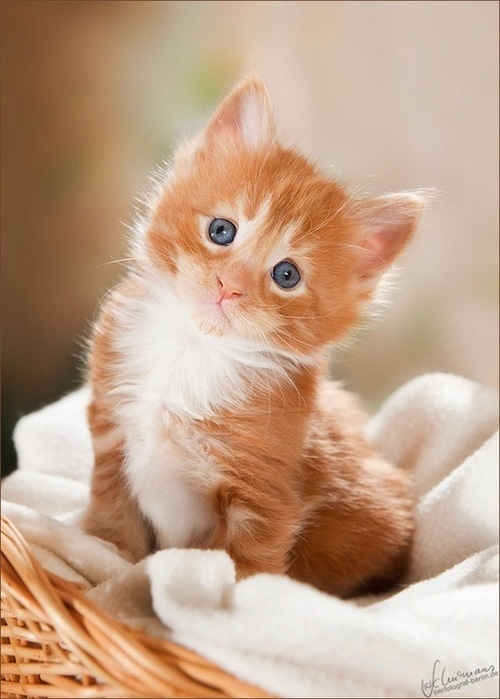
\includegraphics[scale=0.17,trim={0 3.9cm 0 3cm},clip=true,height=3cm]{images/CatImage.jpg}};
	\draw[step=0.5cm,color=gray] (-1.5,-1.5) grid (1.5,1.5);
	\foreach \y in {+0.75,+0.25,-0.25,-0.75}
	\foreach \x in {-0.75,-0.25,0.25,0.75}
	\node at (\x,\y) {$\cdot$};
			
	\foreach \x in {-0.25,0.25,0.75,1.25}
	\node at (\x,1.25) {$\cdot$};
	
	\foreach \x in {-1.25,-0.75,-0.25,0.25,0.75}
	\node at (\x,-1.25) {$\cdot$};
	
	\foreach \y in {-0.75,-0.25,0.25,0.75}{
		\node at (1.25,\y) {$\cdot$};
		\node at (-1.25,\y) {$\cdot$};
	}
	\node at (-1.25,+1.25) {\footnotesize{$\frac{\partial h_i}{\partial x_0}$}};
	\node at (-0.75,+1.25) {\footnotesize{$\frac{\partial h_i}{\partial x_1}$}};
	\node at (+1.25,-1.25) {\footnotesize{$\frac{\partial h_i}{\partial x_{mn}}$}};
			
\end{tikzpicture}	
		% \begin{figure}[hbtp]	
		% 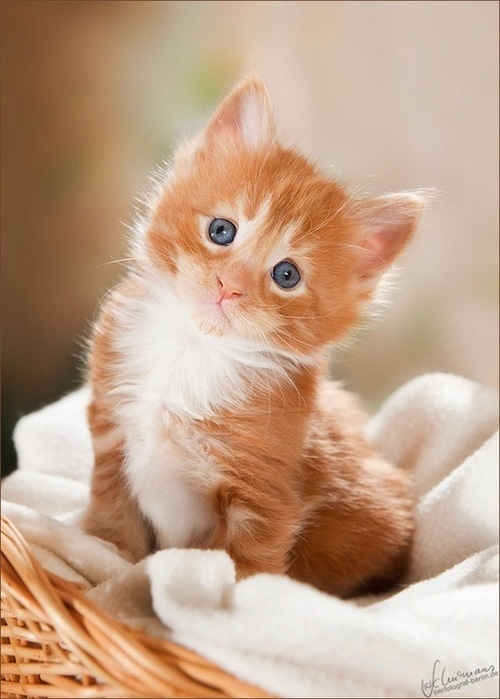
\includegraphics[scale=0.17,trim={0 2cm 0 3cm},clip=true]{images/CatImage.jpg}
		% \end{figure}
		\column{0.5\textwidth}
		\begin{overlayarea}{\textwidth}{\textheight}
			\begin{align*}
				\onslide<1->{\frac{\partial h_j}{\partial x_i} & = 0     & \longrightarrow \text{   no influence}  \\}
				\onslide<2->{\frac{\partial h_j}{\partial x_i} & = large & \longrightarrow \text{ high influence}  \\}
				\onslide<3->{\frac{\partial h_j}{\partial x_i} & = small & \longrightarrow \text{ low influence} } 
			\end{align*}
							
			\begin{itemize}
				\justifying
				\onslide<4->{\item We could just compute these partial derivatives w.r.t all the inputs}
				\onslide<5->{\item And then visualize this gradient matrix as an image itself}								
			\end{itemize}			
		\end{overlayarea}
	\end{columns}
\end{frame}

%%%%%%%%%%%%%%%%%%%%%%%%%%%%%%%%%%%%%%%%%%%%%%%%%%%%%%%%%%%%%%%%%%%%%%%%%%%%%%%%%%%%%%%%%

\begin{frame}
	\begin{columns}
		\column{0.5\textwidth}
		\centering
		\only<1>{
			\begin{tikzpicture}[scale=0.8,transform shape]

\tikzstyle{input_neuron}=[circle,draw=red!50,fill=red!10,thick,minimum size=5mm]
\tikzstyle{input_neuron1}=[circle,draw=yellow!50,fill=yellow,thick,minimum size=5mm]
\tikzstyle{hidden_neuron}=[circle,draw=blue!50,fill=cyan!10,thick,minimum size=5mm]
\tikzstyle{hidden_neuron1}=[circle,draw=yellow!50,fill=yellow,thick,minimum size=5mm]
\tikzstyle{output_neuron}=[circle,draw=green!50,fill=green!10,thick,minimum size=5mm]
\tikzstyle{bias_neuron}=[circle,draw=red!50,fill=red!10,thick,minimum size=2mm]
\tikzstyle{bias_hidden_neuron}=[circle,draw=blue!50,fill=cyan!10,thick,minimum size=2mm]
\tikzstyle{bias_hidden_neuron_hi}=[circle,draw=orange,fill=cyan!10,thick,minimum size=2mm]
\tikzstyle{bias_hidden_neuron_hi_old}=[circle,draw=yellow,fill=cyan!10,thick,minimum size=2mm]
\tikzstyle{input}=[circle,draw=black!50,fill=black!20,thick,minimum size=6mm]

\node [input_neuron] (B) at (-4.0,1){};
\node [input_neuron] (C) at (-3,1){};
\node [input_neuron] (D) at (-2,1){};
\node [input_neuron] (E) at (-1,1){};
\node [input_neuron] (F) at (0,1){};
\node [input_neuron] (G) at (1,1){};
\only<1->{\node [input_neuron] (H) at (2,1){};}
\only<2->{\node [input_neuron1] (H) at (2,1){\tiny $x_i$};}
\node [input_neuron] (I) at (3,1){};
\node [input_neuron] (J) at (4,1){};


\node [rectangle, draw=red, minimum width=90mm, minimum height=6mm] at (0,1){};
\node [hidden_neuron] (O) at (2,2.7){};
\node [hidden_neuron] (N) at (1,2.7){};
\node [hidden_neuron] (M) at (-1,2.7){};
\node [hidden_neuron] (L) at (-2,2.7){};


\node [hidden_neuron] (Oo) at (-3,4){};
\node [hidden_neuron] (Nn) at (-2,4){};
\node [hidden_neuron] (Mm) at (-1,4){};
\only<2->{\node [hidden_neuron1] (Zz) at (0,4){\tiny $h_j$};}
\only<1>{\node [hidden_neuron] (Zz) at (0,4){};}
\node [hidden_neuron] (Ll) at (1,4){};
\node [hidden_neuron] (Xx) at (2,4){};
\node [hidden_neuron] (Yy) at (3,4){};

\node [output_neuron] (To) at (2,5.3){};
\node [output_neuron] (Tp) at (1,5.3){};
\node [output_neuron] (Tq) at (0,5.3){};
\node [output_neuron] (Tr) at (-1,5.3){};
\node [output_neuron] (Ts) at (-2,5.3){};
\onslide<1->{
	
	\draw [->] (B) -- (L);
	\draw [->] (C) -- (L);

	\draw [->] (E) -- (L);




	\draw [->] (C) -- (M);
	\draw [->] (D) -- (M);

	\draw [->] (F) -- (M);
	\draw [->] (G) -- (M);
	\draw [->] (E) -- (N);
	\draw [->] (F) -- (N);
	\draw [->] (H) -- (N);
	\draw [->] (I) -- (N);


	\draw [->] (F) -- (O);
	\draw [->] (G) -- (O);
	\draw [->] (I) -- (O);
	\draw [->] (J) -- (O);

	\draw [->] (L) -- (Oo);
	
	\draw [->] (L) -- (Nn);	
	
	\draw [->] (L) -- (Xx);
	\draw [->] (L) -- (Yy);
	\draw [->] (L) -- (Zz);



	\draw [->] (M) -- (Oo);
	\draw [->] (M) -- (Mm);	
	
	\draw [->] (M) -- (Ll);
	\draw [->] (M) -- (Xx);
	\draw [->] (M) -- (Yy);
	



	
	\draw [->] (N) -- (Mm);	
	\draw [->] (N) -- (Nn);	
	
	\draw [->] (N) -- (Xx);
	
	\draw [->] (N) -- (Zz);



	
	\draw [->] (O) -- (Mm);	
	\draw [->] (O) -- (Nn);	
	
	\draw [->] (O) -- (Xx);
	\draw [->] (O) -- (Yy);
	
	\draw [->] (Ll) -- (To);
	\draw [->] (Ll) -- (Tp);
	\draw [->] (Ll) -- (Tq);
	\draw [->] (Ll) -- (Tr);
	\draw [->] (Ll) -- (Ts);


	\draw [->] (Mm) -- (To);
	\draw [->] (Mm) -- (Tp);
	\draw [->] (Mm) -- (Tq);
	\draw [->] (Mm) -- (Tr);
	\draw [->] (Mm) -- (Ts);

	\draw [->] (Nn) -- (To);
	\draw [->] (Nn) -- (Tp);
	\draw [->] (Nn) -- (Tq);
	\draw [->] (Nn) -- (Tr);
	\draw [->] (Nn) -- (Ts);

	\draw [->] (Mm) -- (To);
	\draw [->] (Mm) -- (Tp);
	\draw [->] (Mm) -- (Tq);
	\draw [->] (Mm) -- (Tr);
	\draw [->] (Mm) -- (Ts);

	\draw [->] (Nn) -- (To);
	\draw [->] (Nn) -- (Tp);
	\draw [->] (Nn) -- (Tq);
	\draw [->] (Nn) -- (Tr);
	\draw [->] (Nn) -- (Ts);


	\draw [->] (Oo) -- (To);
	\draw [->] (Oo) -- (Tp);
	\draw [->] (Oo) -- (Tq);
	\draw [->] (Oo) -- (Tr);
	\draw [->] (Oo) -- (Ts);

	\draw [->] (Xx) -- (To);
	\draw [->] (Xx) -- (Tp);
	\draw [->] (Xx) -- (Tq);
	\draw [->] (Xx) -- (Tr);
	\draw [->] (Xx) -- (Ts);

	\draw [->] (Yy) -- (To);
	\draw [->] (Yy) -- (Tp);
	\draw [->] (Yy) -- (Tq);
	\draw [->] (Yy) -- (Tr);
	\draw [->] (Yy) -- (Ts);



	\draw [->] (Zz) -- (To);
	\draw [->] (Zz) -- (Tp);
	\draw [->] (Zz) -- (Tq);
	\draw [->] (Zz) -- (Tr);
	\draw [->] (Zz) -- (Ts);

	\draw [->, line width=2, color=red] (0,-0.2)-- (0,0.75);
	\node [] at (1,0.25){\footnotesize flatten};
}
\onslide<1->{
	
	\draw [->,color=blue] (B) -- (L);
	\draw [->,color=blue] (C) -- (L);

	\draw [->,color=blue] (E) -- (L);
	\draw [->,color=blue] (F) -- (L);

}

\onslide<1->{
	
	\draw [->,color=blue] (C) -- (M);
	\draw [->,color=blue] (D) -- (M);

	\draw [->,color=blue] (F) -- (M);
	\draw [->,color=blue] (G) -- (M);
}

\onslide<1->{
	
	\draw [->,color=blue] (E) -- (N);
	\draw [->,color=blue] (F) -- (N);

	\draw [->,color=blue] (H) -- (N);
	\draw [->,color=blue] (I) -- (N);


}

\onslide<1->{
	
	\draw [->,color=blue] (F) -- (O);
	\draw [->,color=blue] (I) -- (O);

	\draw [->,color=blue] (G) -- (O);
	\draw [->,color=blue] (J) -- (O);


}
\end{tikzpicture}


			%\vspace{-0.5cm}
			\begin{tikzpicture}
	\node at (+0.0,-0.0) (cat)  { 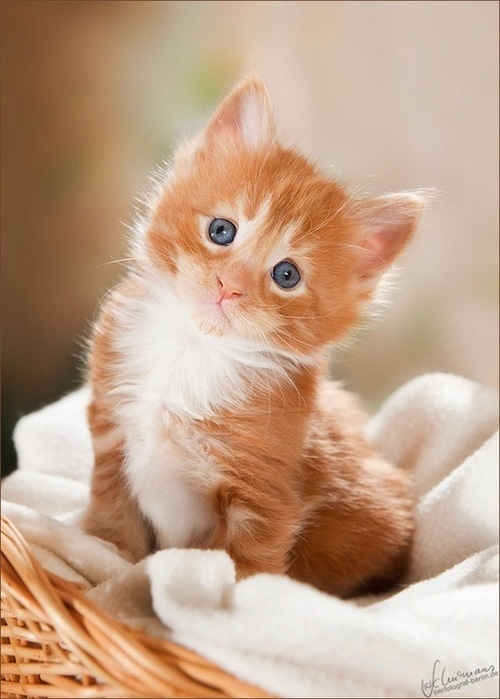
\includegraphics[scale=0.17,trim={0 3.9cm 0 3cm},clip=true,height=3cm]{images/CatImage.jpg}};
	\draw[step=0.5cm,color=gray] (-1.5,-1.5) grid (1.5,1.5);
	\foreach \y in {+0.75,+0.25,-0.25,-0.75}
	\foreach \x in {-0.75,-0.25,0.25,0.75}
	\node at (\x,\y) {$\cdot$};
			
	\foreach \x in {-0.25,0.25,0.75,1.25}
	\node at (\x,1.25) {$\cdot$};
	
	\foreach \x in {-1.25,-0.75,-0.25,0.25,0.75}
	\node at (\x,-1.25) {$\cdot$};
	
	\foreach \y in {-0.75,-0.25,0.25,0.75}{
		\node at (1.25,\y) {$\cdot$};
		\node at (-1.25,\y) {$\cdot$};
	}
	\node at (-1.25,+1.25) {\footnotesize{$x_0$}};
	\node at (-0.75,+1.25) {\footnotesize{$x_1$}};
	\node at (+1.25,-1.25) {\footnotesize{$x_{mn}$}};
			
\end{tikzpicture}	
		}
		\only<2->{
			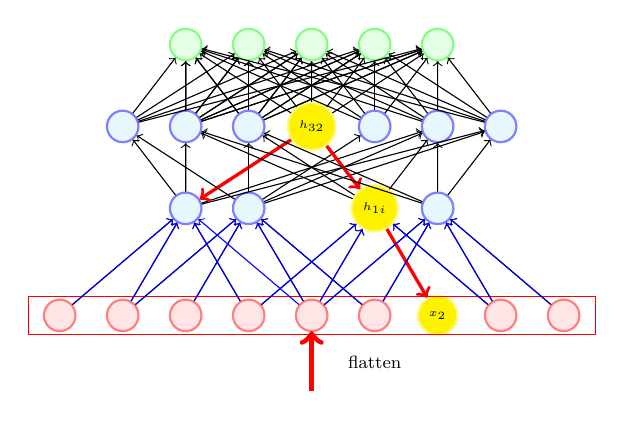
\begin{tikzpicture}[scale=0.8,transform shape]

\tikzstyle{input_neuron}=[circle,draw=red!50,fill=red!10,thick,minimum size=5mm]
\tikzstyle{input_neuron1}=[circle,draw=yellow!50,fill=yellow,thick,minimum size=5mm]
\tikzstyle{hidden_neuron}=[circle,draw=blue!50,fill=cyan!10,thick,minimum size=5mm]
\tikzstyle{hidden_neuron1}=[circle,draw=yellow!50,fill=yellow,thick,minimum size=5mm]
\tikzstyle{output_neuron}=[circle,draw=green!50,fill=green!10,thick,minimum size=5mm]
\tikzstyle{bias_neuron}=[circle,draw=red!50,fill=red!10,thick,minimum size=2mm]
\tikzstyle{bias_hidden_neuron}=[circle,draw=blue!50,fill=cyan!10,thick,minimum size=2mm]
\tikzstyle{bias_hidden_neuron_hi}=[circle,draw=orange,fill=cyan!10,thick,minimum size=2mm]
\tikzstyle{bias_hidden_neuron_hi_old}=[circle,draw=yellow,fill=cyan!10,thick,minimum size=2mm]
\tikzstyle{input}=[circle,draw=black!50,fill=black!20,thick,minimum size=6mm]

\node [input_neuron] (B) at (-4.0,1){};
\node [input_neuron] (C) at (-3,1){};
\node [input_neuron] (D) at (-2,1){};
\node [input_neuron] (E) at (-1,1){};
\node [input_neuron] (F) at (0,1){};
\node [input_neuron] (G) at (1,1){};
\node [input_neuron1] (H) at (2,1){\tiny $x_2$};
\node [input_neuron] (I) at (3,1){};
\node [input_neuron] (J) at (4,1){};


\node [rectangle, draw=red, minimum width=90mm, minimum height=6mm] at (0,1){};
\node [hidden_neuron] (O) at (2,2.7){};
\node [hidden_neuron] (N) at (1,2.7){};
\onslide<2->{\node [hidden_neuron1] (N) at (1,2.7){\tiny $h_{1i}$};}
\node [hidden_neuron] (M) at (-1,2.7){};
\node [hidden_neuron] (L) at (-2,2.7){};


\node [hidden_neuron] (Oo) at (-3,4){};
\node [hidden_neuron] (Nn) at (-2,4){};
\node [hidden_neuron] (Mm) at (-1,4){};
\node [hidden_neuron1] (Zz) at (0,4){\tiny $h_{32}$};

\node [hidden_neuron] (Ll) at (1,4){};
\node [hidden_neuron] (Xx) at (2,4){};
\node [hidden_neuron] (Yy) at (3,4){};

\node [output_neuron] (To) at (2,5.3){};
\node [output_neuron] (Tp) at (1,5.3){};
\node [output_neuron] (Tq) at (0,5.3){};
\node [output_neuron] (Tr) at (-1,5.3){};
\node [output_neuron] (Ts) at (-2,5.3){};
\onslide<1->{
	
	\draw [->] (B) -- (L);
	\draw [->] (C) -- (L);

	\draw [->] (E) -- (L);




	\draw [->] (C) -- (M);
	\draw [->] (D) -- (M);

	\draw [->] (F) -- (M);
	\draw [->] (G) -- (M);
	\draw [->] (E) -- (N);
	\draw [->] (F) -- (N);
	\draw [->, color=red, line width=1.2] (N) -- (H);
	\draw [->] (I) -- (N);


	\draw [->] (F) -- (O);
	\draw [->] (G) -- (O);
	\draw [->] (I) -- (O);
	\draw [->] (J) -- (O);

	\draw [->] (L) -- (Oo);
	
	\draw [->] (L) -- (Nn);	
	
	\draw [->] (L) -- (Xx);
	\draw [->] (L) -- (Yy);
	\draw [->,color=red, line width=1.2] (Zz) -- (L);



	\draw [->] (M) -- (Oo);
	\draw [->] (M) -- (Mm);	
	
	\draw [->] (M) -- (Ll);
	\draw [->] (M) -- (Xx);
	\draw [->] (M) -- (Yy);
	



	
	\draw [->] (N) -- (Mm);	
	\draw [->] (N) -- (Nn);	
	
	\draw [->] (N) -- (Xx);
	
	\draw [->,color=red, line width=1.2] (Zz) -- (N);



	
	\draw [->] (O) -- (Mm);	
	\draw [->] (O) -- (Nn);	
	
	\draw [->] (O) -- (Xx);
	\draw [->] (O) -- (Yy);
	
	\draw [->] (Ll) -- (To);
	\draw [->] (Ll) -- (Tp);
	\draw [->] (Ll) -- (Tq);
	\draw [->] (Ll) -- (Tr);
	\draw [->] (Ll) -- (Ts);


	\draw [->] (Mm) -- (To);
	\draw [->] (Mm) -- (Tp);
	\draw [->] (Mm) -- (Tq);
	\draw [->] (Mm) -- (Tr);
	\draw [->] (Mm) -- (Ts);

	\draw [->] (Nn) -- (To);
	\draw [->] (Nn) -- (Tp);
	\draw [->] (Nn) -- (Tq);
	\draw [->] (Nn) -- (Tr);
	\draw [->] (Nn) -- (Ts);

	\draw [->] (Mm) -- (To);
	\draw [->] (Mm) -- (Tp);
	\draw [->] (Mm) -- (Tq);
	\draw [->] (Mm) -- (Tr);
	\draw [->] (Mm) -- (Ts);

	\draw [->] (Nn) -- (To);
	\draw [->] (Nn) -- (Tp);
	\draw [->] (Nn) -- (Tq);
	\draw [->] (Nn) -- (Tr);
	\draw [->] (Nn) -- (Ts);


	\draw [->] (Oo) -- (To);
	\draw [->] (Oo) -- (Tp);
	\draw [->] (Oo) -- (Tq);
	\draw [->] (Oo) -- (Tr);
	\draw [->] (Oo) -- (Ts);

	\draw [->] (Xx) -- (To);
	\draw [->] (Xx) -- (Tp);
	\draw [->] (Xx) -- (Tq);
	\draw [->] (Xx) -- (Tr);
	\draw [->] (Xx) -- (Ts);

	\draw [->] (Yy) -- (To);
	\draw [->] (Yy) -- (Tp);
	\draw [->] (Yy) -- (Tq);
	\draw [->] (Yy) -- (Tr);
	\draw [->] (Yy) -- (Ts);



	\draw [->] (Zz) -- (To);
	\draw [->] (Zz) -- (Tp);
	\draw [->] (Zz) -- (Tq);
	\draw [->] (Zz) -- (Tr);
	\draw [->] (Zz) -- (Ts);

	\draw [->, line width=2, color=red] (0,-0.2)-- (0,0.75);
	\node [] at (1,0.25){\footnotesize flatten};
}
\onslide<1->{
	
	\draw [->,color=blue] (B) -- (L);
	\draw [->,color=blue] (C) -- (L);

	\draw [->,color=blue] (E) -- (L);
	\draw [->,color=blue] (F) -- (L);

}

\onslide<1->{
	
	\draw [->,color=blue] (C) -- (M);
	\draw [->,color=blue] (D) -- (M);

	\draw [->,color=blue] (F) -- (M);
	\draw [->,color=blue] (G) -- (M);
}

\onslide<1->{
	
	\draw [->,color=blue] (E) -- (N);
	\draw [->,color=blue] (F) -- (N);


	\draw [->,color=blue] (I) -- (N);


}

\onslide<1->{
	
	\draw [->,color=blue] (F) -- (O);
	\draw [->,color=blue] (I) -- (O);

	\draw [->,color=blue] (G) -- (O);
	\draw [->,color=blue] (J) -- (O);


}
\end{tikzpicture}


			%\vspace{-0.5cm}
			\begin{tikzpicture}
	\node at (+0.0,-0.0) (cat)  { 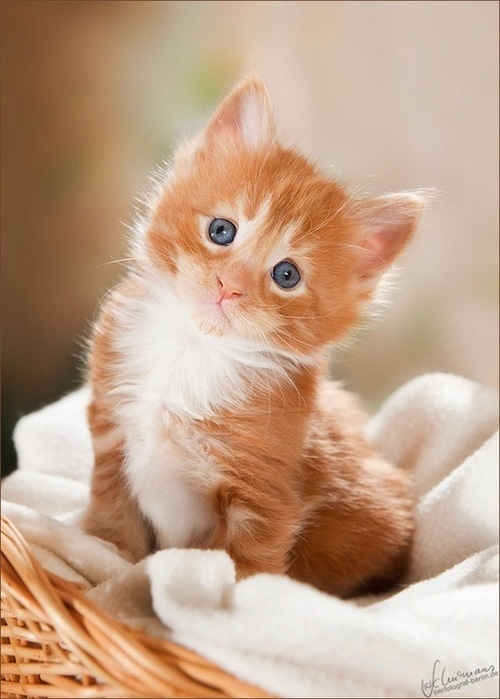
\includegraphics[scale=0.17,trim={0 3.9cm 0 3cm},clip=true,height=3cm]{images/CatImage.jpg}};
	\draw[step=0.5cm,color=gray] (-1.5,-1.5) grid (1.5,1.5);
	\foreach \y in {+0.75,+0.25,-0.25,-0.75}
	\foreach \x in {-0.75,-0.25,0.25,0.75}
	\node at (\x,\y) {$\cdot$};
			
	\foreach \x in {-0.25,0.25,0.75,1.25}
	\node at (\x,1.25) {$\cdot$};
	
	\foreach \x in {-1.25,-0.75,-0.25,0.25,0.75}
	\node at (\x,-1.25) {$\cdot$};
	
	\foreach \y in {-0.75,-0.25,0.25,0.75}{
		\node at (1.25,\y) {$\cdot$};
		\node at (-1.25,\y) {$\cdot$};
	}
	\node at (-1.25,+1.25) {\footnotesize{$x_0$}};
	\node at (-0.75,+1.25) {\footnotesize{$x_1$}};
	\node at (+1.25,-1.25) {\footnotesize{$x_{mn}$}};
			
\end{tikzpicture}	
		}	
		
		\column{0.5\textwidth}
		\begin{overlayarea}{\textwidth}{\textheight}
			\begin{itemize}
				\justifying
				\onslide<1->{\item But how do we compute these gradients?}
				\onslide<2->{\item Recall that we can represent CNNs by feedforward neural network}
				\onslide<3->{\item Then we already know how to compute influences (gradient) using backpropogation}
				\onslide<4->{\item For example, we know how to backprop the gradients till the first hidden layer}
				\onslide<5->{
					\footnotesize{
						\begin{align*}
							\frac{\partial h_{32}}{\partial x_{2}} & = \sum_{i=1}^{3} \frac{\partial h_{32}}{\partial h_{1i}} \frac{\partial h_{1i}}{\partial x_2} \\
							h_{1i}                                 & = \sum_{j=1}^{4} w_{ji}x_{j}                                                                  \\
							\frac{\partial h_{1i}}{\partial x_2}   & = w_{12}                                                                                      
						\end{align*}
				}}
				
			\end{itemize}
		\end{overlayarea}
	\end{columns}
\end{frame}

%%%%%%%%%%%%%%%%%%%%%%%%%%%%%%%%%%%%%%%%%%%%%%%%%%%%%%%%%%%%%%%%%%%%%%%%%%%%%%%%%%%%%%%%%

\begin{frame}
	\begin{columns}
		\column{0.5\textwidth}
		\centering
		\begin{figure}[hbtp]
			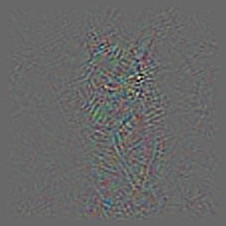
\includegraphics[scale=0.4]{images/2_4_1.png}
		\end{figure}
		
			
		\column{0.5\textwidth}
		\begin{overlayarea}{\textwidth}{\textheight}
			\begin{itemize}
				\justifying
				\item<1-> This is what we get if we compute the gradients and plot it as an image
				\onslide<2->{\item The above procedure does not show very sharp influences }
				
				\onslide<3->{\item Springenberg et al. proposed ``guided back propagation'' which gives a better idea about the influences}
			\end{itemize}
		\end{overlayarea}
	\end{columns}
\end{frame}
